\documentclass[border=6pt,tikz]{standalone}
\usepackage{tikz}
\usepackage{amsmath,amssymb}
\usetikzlibrary{arrows.meta,positioning,fit,backgrounds,calc,shapes.geometric,decorations.pathreplacing,patterns}
\definecolor{ink}{HTML}{1B2430}
\definecolor{muted}{HTML}{6B7785}
\definecolor{accent}{HTML}{2F6FB5}
\definecolor{accent2}{HTML}{C1611F}
\definecolor{good}{HTML}{2E7D5B}
\definecolor{soft}{HTML}{EDF2F7}
\definecolor{soft2}{HTML}{FBEDE2}
\definecolor{soft3}{HTML}{E6F0E9}
\tikzset{
  box/.style={draw=ink,line width=.7pt,rounded corners=2pt,fill=soft,inner sep=4pt,align=center,font=\sffamily\small},
  boxa/.style={box,fill=soft2},
  boxb/.style={box,fill=soft3},
  plain/.style={align=center,font=\sffamily\small,text=ink},
  tiny/.style={align=center,font=\sffamily\scriptsize,text=muted},
  ar/.style={-{Stealth[length=2.4mm]},draw=ink,line width=.7pt},
  arm/.style={-{Stealth[length=2.4mm]},draw=muted,line width=.6pt,dashed},
  nd/.style={circle,draw=ink,line width=.7pt,fill=white,minimum size=7mm,inner sep=0pt,font=\sffamily\scriptsize},
  ndf/.style={nd,fill=soft},
  ndt/.style={nd,fill=soft2},
}

\begin{document}
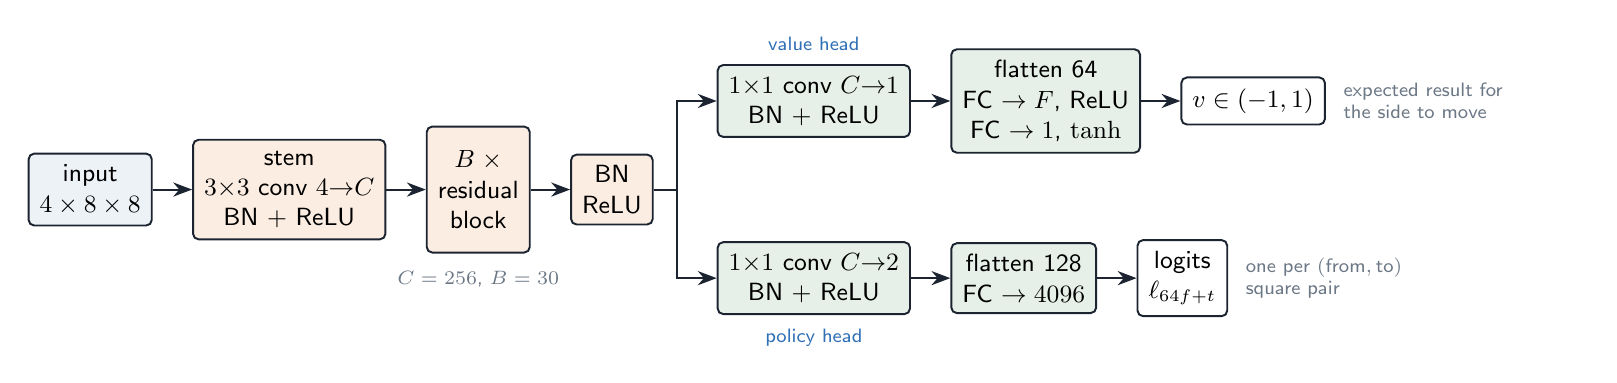
\begin{tikzpicture}[node distance=5mm]
  \node[box] (in) {input\\$4\times8\times8$};
  \node[boxa,right=of in] (stem) {stem\\$3{\times}3$ conv $4{\to}C$\\BN + ReLU};
  \node[boxa,right=of stem,minimum height=16mm] (trunk) {$B\;\times$\\residual\\block};
  \node[boxa,right=of trunk] (obn) {BN\\ReLU};
  \node[plain,right=3mm of obn] (split) {};

  \node[boxb,above right=2mm and 8mm of obn] (vc) {$1{\times}1$ conv $C{\to}1$\\BN + ReLU};
  \node[boxb,right=of vc] (vf) {flatten 64\\FC $\to F$, ReLU\\FC $\to 1$, $\tanh$};
  \node[box,right=of vf,fill=white] (v) {$v\in(-1,1)$};

  \node[boxb,below right=2mm and 8mm of obn] (pc) {$1{\times}1$ conv $C{\to}2$\\BN + ReLU};
  \node[boxb,right=of pc] (pf) {flatten 128\\FC $\to 4096$};
  \node[box,right=of pf,fill=white] (p) {logits\\$\ell_{64f+t}$};

  \draw[ar] (in) -- (stem);
  \draw[ar] (stem) -- (trunk);
  \draw[ar] (trunk) -- (obn);
  \draw[ar] (obn.east) -- ++(3mm,0) |- (vc.west);
  \draw[ar] (obn.east) -- ++(3mm,0) |- (pc.west);
  \draw[ar] (vc) -- (vf); \draw[ar] (vf) -- (v);
  \draw[ar] (pc) -- (pf); \draw[ar] (pf) -- (p);

  \node[tiny,below=1mm of trunk] {$C=256$, $B=30$};
  \node[tiny,above=0.5mm of vc,text=accent] {value head};
  \node[tiny,below=0.5mm of pc,text=accent] {policy head};
  \node[tiny,right=1mm of v,text width=30mm,align=left] {expected result for\\the side to move};
  \node[tiny,right=1mm of p,text width=30mm,align=left] {one per $(\text{from},\text{to})$\\square pair};
\end{tikzpicture}
\end{document}
